% +------------------------------------------------------------------------+
% | Reference manual page: HalfedgeDS.tex
% +------------------------------------------------------------------------+
% | 22.03.1999   Lutz Kettner
% | Package: HalfedgeDS
% | 
\RCSdef{\RCSHalfedgeDSRev}{$Revision$}
\RCSdefDate{\RCSHalfedgeDSDate}{$Date$}
% +------------------------------------------------------------------------+

\ccRefPageBegin

%%RefPage: end of header, begin of main body
% +------------------------------------------------------------------------+


\begin{ccRefConcept}{HalfedgeDS<Traits,Items>}

\ccCreationVariable{hds}
\ccTagFullDeclarations

% +-----------------------------------+
\ccDefinition
  
The concept of a halfedge data structure (abbreviated as \ccRefName, or
\ccc{HDS} for template parameters) defines an edge-centered data structure
capable of maintaining incidence informations of vertices, edges and
faces, for example for planar maps or polyhedral surfaces. It is a
combinatorial data structure, geometric interpretation is added by
classes built on top of the halfedge data structure.

The data structure defined here is known as the
FE-structure~\cite{w-ebdss-85}, as
halfedges~\cite{m-ism-88,bfh-mgedm-95} or as the doubly connected edge
list (DCEL)~\cite{bkos-cgaa-97}, although the original reference for
the DCEL~\cite{mp-fitcp-78} describes a different data structure. The
halfedge data structure can also be seen as one of the variants of the
quad-edge data structure~\cite{gs-pmgsc-85} that supports only
orientable 2-manifolds. In general, the quad-edge data can represent
non-orientable 2-manifolds.  An overview and comparison of these
different data structures together with a thorough description of the
design implemented here can be found in~\cite{k-ugpdd-99}.

Each edge is represented by two halfedges with opposite orientations.
Each halfedge can store a reference to an incident face and an
incident vertex.  For each face and each vertex an incident halfedge
is stored.  Reduced variants of the halfedge data structure can omit
some of these informations, for example the reference to halfedges in
vertices or the storage of vertices at all. See 
Figure~\ccTexHtml{\ref{figureOptionalMethods}}{}\begin{ccHtmlOnly}
  <A HREF="HalfedgeDS.html#figureOptionalMethods"><IMG 
  SRC="cc_ref_up_arrow.gif" ALT="reference arrow" WIDTH="10" HEIGHT="10"></A>
\end{ccHtmlOnly}
for the incidences, the mandatory and optional member functions
possible for vertices, halfedges and faces.

\begin{ccTexOnly}
    \begin{figure}[bht]
        \begin{center}
          \parbox{\textwidth}{%
              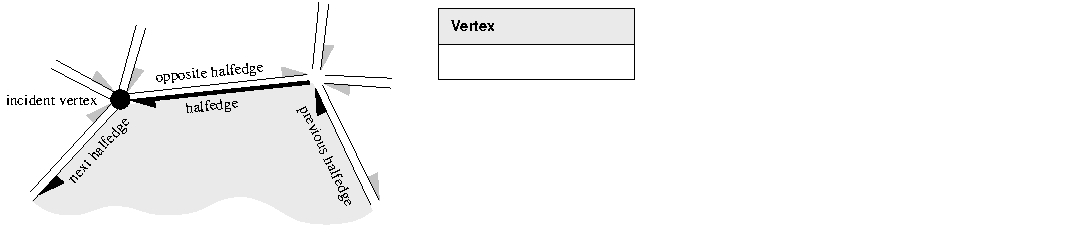
\includegraphics[width=\textwidth]{fig/hds_optional.ips}%
          }
        \end{center}
        \caption{The three classes \protect\ccc{Vertex}, 
          \protect\ccc{Halfedge}, and 
          \protect\ccc{Face} of the halfedge data structure. Member
          functions with shaded background are mandatory. The others
          are optionally supported.}
        \label{figureOptionalMethods}
    \end{figure}
\end{ccTexOnly}

\begin{ccHtmlOnly}
    <CENTER>
    <A NAME="figureOptionalMethods">
    <A HREF="./hds_optional.gif">
        <img src="./hds_optional_small.gif" 
             alt="Class Diagram"></A><BR>
    <A HREF="./hds_optional.gif">Figure:</A>
    The three classes <I>Vertex</I>, <I>Halfedge</I>, and 
          <I>Face</I> of the halfedge data structure. Member
          functions with shaded background are mandatory. The others
          are optionally supported.
    </CENTER>
\end{ccHtmlOnly}

A \ccRefName\ organizes the internal storage of its items.  Examples
are a list-based or an \stl\ vector-based storage. The \ccRefName\ 
possesses most of the characteristics of the container class used
internally, for example the iterator category. An \stl\ vector resizes
automatically when a new item exceeds the reserved space. Since
resizing is an expensive operation for a \ccRefName\ in general and
only possible in a well defined state of the data structure (no
dangling handles), it must be called explicitly in advance for a
\ccRefName\ before inserting new items beyond the current capacity.
Classes built on top of a \ccRefName\ are advised to call the
\ccc{reserve()} member function before creating new items.

% +-----------------------------------+
\ccParameters

A \ccRefName\ is a class template and will be used as argument for
other class templates, for example \ccc{CGAL::Polyhedron_3}. The
template parameters to instantiate the \ccRefName\ will be provided by
this other class template. Therefore, the two template parameters and
their meaning are mandatory. We distinguish between \ccRefName\ and 
an instantiation of \ccRefName.

\ccc{Traits} is a traits class that will be passed to the 
item types in \ccc{Items}. It will not be used in \ccRefName\
itself. \ccc{Items} is a model of the \ccc{HalfedgeDS_Items} concept.

% +-----------------------------------+
\ccTypes

\ccTwo{HalfedgeDS<Traits,Items>:: circulator_category}{}

\ccNestedType{Traits}{traits class.}
\ccGlue
\ccNestedType{Items}{items, model of \ccc{HalfedgeDS_Items} concept.}

\ccNestedType{size_type}{size type of \ccc{HalfedgeDS}.}
\ccGlue
\ccNestedType{difference_type}{difference type of \ccc{HalfedgeDS}.}
\ccGlue
\ccNestedType{iterator_category}{iterator category of \ccc{HalfedgeDS}
    for all iterators.}

\ccNestedType{Vertex}{vertex, model of \ccc{HalfedgeDS_Vertex} concept.}
\ccGlue
\ccNestedType{Halfedge}{halfedge, model of
                        \ccc{HalfedgeDS_Halfedge} concept.}
\ccGlue
\ccNestedType{Face}{face, model of \ccc{HalfedgeDS_Face} concept.}

The following handles and iterators have appropriate
non-mutable counterparts, i.e.~\ccc{const_handle} and
\ccc{const_iterator}. The mutable types are
assignable to their non-mutable counterparts. The iterators are
assignable to the respective handle types. Wherever the handles appear
in function parameter lists, the corresponding iterators can be used as
well. {\bf Note:} The handle types must have a default constructor
that creates a unique and always the same handle value. It will be
used in analogy to \ccc{NULL} for pointers.

\ccNestedType{Vertex_handle}{handle to vertex.}
\ccGlue
\ccNestedType{Halfedge_handle}{handle to halfedge.}
\ccGlue
\ccNestedType{Face_handle}{handle to face.}

\ccNestedType{Vertex_iterator}{iterator over all vertices.}
\ccGlue
\ccNestedType{Halfedge_iterator}{iterator over all halfedges.}
\ccGlue
\ccNestedType{Face_iterator}{iterator over all faces.}

% +-----------------------------------+
\begin{ccAdvanced}
\ccHeading{Types for Tagging Optional Features}

\ccTwo{HalfedgeDS<Traits,Items>:: Supports_vertex_halfedge}{}

The following types are equal to either \ccStyle{CGAL::Tag_true} or
\ccStyle{CGAL::Tag_false}, depending on whether the named feature is
supported or not.

\ccNestedType{Supports_vertex_halfedge}{\ccc{Vertex::halfedge()}.}
\ccGlue
\ccNestedType{Supports_halfedge_prev}{\ccc{Halfedge::prev()}.}
\ccGlue
\ccNestedType{Supports_halfedge_vertex}{\ccc{Halfedge::vertex()}.}
\ccGlue
\ccNestedType{Supports_halfedge_face}{\ccc{Halfedge::face()}.}
\ccGlue
\ccNestedType{Supports_face_halfedge}{\ccc{Face::halfedge()}.}
\ccGlue
\ccNestedType{Supports_removal}{supports removal of individual elements.}

The following dependencies among these options must be regarded:

Vertices are supported $\Longleftrightarrow$
\ccc{Supports_halfedge_vertex} $\equiv$ \ccc{CGAL::Tag_true}.
\\
Faces are supported $\Longleftrightarrow$
\ccc{Supports_halfedge_face} $\equiv$ \ccc{CGAL::Tag_true}.
\\
\ccc{Supports_vertex_halfedge} $\equiv$ \ccc{CGAL::Tag_true} $\Longrightarrow$
\ccc{Supports_halfedge_vertex} $\equiv$ \ccc{CGAL::Tag_true}.
\\
\ccc{Supports_vertex_point} $\equiv$ \ccc{CGAL::Tag_true} $\Longrightarrow$
\ccc{Supports_halfedge_vertex} $\equiv$ \ccc{CGAL::Tag_true}.
\\
\ccc{Supports_face_halfedge} $\equiv$ \ccc{CGAL::Tag_true} $\Longrightarrow$
\ccc{Supports_halfedge_face} $\equiv$ \ccc{CGAL::Tag_true}.


\end{ccAdvanced}

% +-----------------------------------+
\ccHeading{Static Member Functions}
\ccThree{static Halfedge_const_handle HalfedgeDS:::}{function}{}

The following static member functions of \ccRefName\ return the appropriate
handle to an item given a pointer to this item.

\ccFunction{static Vertex_handle 
  HalfedgeDS::vertex_handle( Vertex* v);}{}
\ccGlue
\ccFunction{static Vertex_const_handle 
  HalfedgeDS::vertex_handle( const Vertex* v);}{}

\ccFunction{static Halfedge_handle 
  HalfedgeDS::halfedge_handle( Halfedge* h);}{}
\ccGlue
\ccFunction{static Halfedge_const_handle 
  HalfedgeDS::halfedge_handle( const Halfedge* h);}{}

\ccFunction{static Face_handle 
  HalfedgeDS::face_handle( Face* f);}{}
\ccGlue
\ccFunction{static Face_const_handle 
  HalfedgeDS::face_handle( const Face* f);}{}

% +-----------------------------------+
\ccCreation
\ccThree{HalfedgeDS<Traits,Items>& }{functionfoo}{}
\ccThreeToTwo

\ccConstructor{HalfedgeDS();}{empty halfedge data structure.}

\ccConstructor{HalfedgeDS( size_type v, size_type h, size_type f);}
    {storage reserved for $v$ vertices, $h$ halfedges, and $f$ faces.}

\ccTagDefaults
\ccConstructor{HalfedgeDS( const HalfedgeDS<Traits,Items>& hds2);}
    {copy constructor. \ccPrecond \ccc{hds2} contains no dangling handles.}

\ccMethod{HalfedgeDS<Traits,Items>& 
          operator=( const HalfedgeDS<Traits,Items>& hds2);}
    {assignment operator. \ccPrecond \ccc{hds2} contains no dangling handles.}

\ccMethod{void reserve( size_type v, size_type h, size_type f);}
    {reserves storage for $v$ vertices, $h$ halfedges, and $f$ faces.
     If all capacities are already greater or equal than the requested sizes
     nothing happens. Otherwise, \ccVar\ will be resized and all handles, 
     iterators and circulators invalidate.}


% +-----------------------------------+
\ccHeading{Access Member Functions}
\ccThree{Halfedge_iterator}{hds.capacity_of_halfedges();}{}

\ccMethod{Size size_of_vertices() const;}{number of vertices.}
\ccGlue
\ccMethod{Size size_of_halfedges() const;}{number of halfedges.}
\ccGlue
\ccMethod{Size size_of_faces() const;}{number of faces.}
\ccGlue
\ccMethod{Size capacity_of_vertices() const;}{space reserved for vertices.}
\ccGlue
\ccMethod{Size capacity_of_halfedges() const;}{space reserved for halfedges.}
\ccGlue
\ccMethod{Size capacity_of_faces() const;}{space reserved for faces.}
\ccGlue
\ccMethod{size_t bytes() const;}{bytes used for \ccVar.}
\ccGlue
\ccMethod{size_t bytes_reserved() const;}{bytes reserved for \ccVar.}

The following member functions return the non-mutable iterator if
\ccVar\ is declared const.

\ccMethod{Vertex_iterator    vertices_begin();}{iterator over all vertices.}
\ccGlue
\ccMethod{Vertex_iterator    vertices_end();}{}
\ccGlue
\ccMethod{Halfedge_iterator  halfedges_begin();}{iterator over all halfedges}
\ccGlue
\ccMethod{Halfedge_iterator  halfedges_end();}{}
\ccGlue
\ccMethod{Face_iterator     faces_begin();}{iterator over all faces.}
\ccGlue
\ccMethod{Face_iterator     faces_end();}{}

% +-----------------------------------+
\ccHeading{Insertion}
\ccTagFullDeclarations

Note that the vertex-related and the face-related member functions may
not be provided for a \ccRefName\ that does not support vertices or
faces respectively.

\ccMethod{Vertex_handle vertices_push_back( const Vertex& v);}
    {appends a copy of $v$ to \ccc{hds}. Returns a handle of the new vertex.}
\ccGlue
\ccMethod{Halfedge_handle edges_push_back( const Halfedge& h, 
                                           const Halfedge& g);}
    {appends a copy of $h$ and a copy of $g$ to \ccc{hds} and makes the
     copies the opposite halfedge of each other. 
     Returns a handle of the halfedge copy of $h$.}
\ccGlue
\ccMethod{Halfedge_handle edges_push_back( const Halfedge& h);}
    {appends a copy of $h$ and a copy of $h->opposite()$ to \ccc{hds} 
     and makes the copies the opposite halfedge of each other. 
     Returns a handle of the halfedge copy of $h$. \ccPrecond
     \ccc{h->opposite()} denotes a halfedge.}
\ccGlue
\ccMethod{Face_handle faces_push_back( const Face& f);}
    {appends a copy of $f$ to \ccc{hds}. Returns a handle of the new face.}


% +-----------------------------------+
\ccHeading{Removal}
\ccThree{Halfe}{dge_iteratorhds.capacity_of_halfedges();}{}

Erasing single elements is optional and indicated with the type tag
\ccc{Supports_removal}. The \ccc{pop_back} member functions and the
deletion of all items are mandatory, except that the vertex-related
and the face-related member functions may not be provided for a
\ccRefName\ that does not support vertices or faces respectively.


\ccMethod{void vertices_pop_front();}{
    removes the first vertex if vertices are supported and
    \ccc{Supports_removal} $\equiv$ \ccc{CGAL::Tag_true}.}
\ccGlue
\ccMethod{void vertices_pop_back();}{
    removes the last vertex if vertices are supported.}
\ccGlue
\ccMethod{void vertices_erase( Vertex_handle v);}{
    removes the vertex $v$ if vertices are supported and
    \ccc{Supports_removal} $\equiv$ \ccc{CGAL::Tag_true}.}
\ccGlue
\ccMethod{void vertices_erase( Vertex_handle first, Vertex_handle last);}{
    removes the range of vertices $[\ccc{first},\ccc{last})$ if vertices 
    are supported and \ccc{Supports_removal} $\equiv$ \ccc{CGAL::Tag_true}.}

\ccMethod{void edges_pop_front();}{
    removes the first two halfedges if halfedges are supported and
    \ccc{Supports_removal} $\equiv$ \ccc{CGAL::Tag_true}.}
\ccGlue
\ccMethod{void edges_pop_back();}{
    removes the last two halfedges if halfedges are supported.}
\ccGlue
\ccMethod{void edges_erase( Halfedge_handle h);}{
    removes the pair of opposite halfedges $h$ and \ccc{h->opposite()}
    if halfedges are supported and
    \ccc{Supports_removal} $\equiv$ \ccc{CGAL::Tag_true}.}
\ccGlue
\ccMethod{void edges_erase( Halfedge_handle first, Halfedge_handle last);}{
    removes the range of edges $[\ccc{first},\ccc{last})$ if halfedges 
    are supported and \ccc{Supports_removal} $\equiv$ \ccc{CGAL::Tag_true}.}

\ccMethod{void faces_pop_front();}{
    removes the first face if faces are supported and
    \ccc{Supports_removal} $\equiv$ \ccc{CGAL::Tag_true}.}
\ccGlue
\ccMethod{void faces_pop_back();}{
    removes the last face if faces are supported.}
\ccGlue
\ccMethod{void faces_erase( Face_handle f);}{
    removes the face $f$ if faces are supported and
    \ccc{Supports_removal} $\equiv$ \ccc{CGAL::Tag_true}.}
\ccGlue
\ccMethod{void faces_erase( Face_handle first, Face_handle last);}{
    removes the range of faces $[\ccc{first},\ccc{last})$ if faces are 
    supported and \ccc{Supports_removal} $\equiv$ \ccc{CGAL::Tag_true}.}

\ccMethod{void erase_all();}{removes all elements.}

% +-----------------------------------+
\ccHeading{Operations with Border Halfedges}

\begin{ccAdvanced}
  
The following notion of border halfedges is particular useful where
the halfedge data structure is used to model surfaces with open
regions.  Halfedges incident to an open region are called {\em
  border halfedges}. A halfedge is a {\em border edge\/} if the
halfedge itself or its opposite halfedge is a border halfedge. The
only requirement to work with border halfedges is that the
\ccc{Halfedge} class provides a member function \ccc{is_border()}
returning a \ccc{bool}. Usually, the halfedge data structure
supports faces and the value of the default constructor of the face
handle will indicate a border halfedge, but this may not be the only
possibility. The \ccc{is_border()} predicate divides the edges into
two classes, the border edges and the non-border edges. The
following normalization reorganizes the sequential storage of the
edges such that the non-border edges precede the border edges, and
that for each border edge the latter of the two halfedges is a
border halfedge (the first one might be a border halfedge too). The
normalization stores the number of border halfedges, as well as the
halfedge iterator where the border edges start at, within the
halfedge data structure.  These values will be invalid after further
halfedge insertions or removals and changes in the border status of 
a halfedge. The is no automatic update required.

\ccThree{Halfedge_iterator}{hds.size_of;}{}

\ccMethod{void   normalize_border();}
    {sorts halfedges such that the non-border edges precede the
     border edges. For each border edge that is incident to a face,
     the halfedge iterator will reference the halfedge incident to the
     face right before the halfedge incident to the open region.}

\ccMethod{Size size_of_border_halfedges() const;}
    {number of border halfedges. An edge with no incident face
      counts as two border halfedges.
    \ccPrecond \ccc{normalize_border()} has been called and no
    halfedge insertion or removal and no change in border
    status of the halfedges have occurred since then.}

\ccMethod{Size size_of_border_edges() const;}
    {number of border edges. If \ccc{size_of_border_edges()} is equal
    to \ccc{size_of_border_halfedges()} all border edges are incident to
    a face on one side and to an open region on the other side.
    \ccPrecond \ccc{normalize_border()} has been called and no
    halfedge insertion or removal and no change in border
    status of the halfedges have occurred since then.}

\ccMethod{Halfedge_iterator  border_halfedges_begin();}
    {halfedge iterator starting with the border edges. The range
      [\ccStyle{halfedges_begin(), border_halfedges_begin()}) denotes
    all non-border edges. The range
    [\ccStyle{border_halfedges_begin(), halfedges_end()}) denotes all
    border edges.
    \ccPrecond \ccc{normalize_border()} has been called and no
    halfedge insertion or removal and no change in border
    status of the halfedges have occurred since then.}

\end{ccAdvanced}


% +-----------------------------------+
\ccHasModels

\ccc{CGAL::HalfedgeDS_default<Traits>},
\ccc{CGAL::HalfedgeDS_using_in_place_list<Traits,Items>},\\
\ccc{CGAL::HalfedgeDS_using_list<Traits,Items>},
\ccc{CGAL::HalfedgeDS_using_vector<Traits,Items>}.

% +-----------------------------------+
\ccSeeAlso

\ccc{HalfedgeDS_Items},
\ccc{CGAL::Polyhedron_3},
\ccc{CGAL::HalfedgeDS_vertex_base<Refs>},\\
\ccc{CGAL::HalfedgeDS_halfedge_base<Refs>},
\ccc{CGAL::HalfedgeDS_face_base<Refs>},\\
\ccc{CGAL::HalfedgeDS_items_decorator<HDS>},
\ccc{CGAL::HalfedgeDS_decorator<HDS>},\\
\ccc{CGAL::HalfedgeDS_const_decorator<HDS>}.

% +-----------------------------------+
\ccImplementation

Classes parameterized with a halfedge data structure, such as
\ccc{CGAL::Polyhedron_3}, need to declare a class template as one of its
template parameters for the \ccRefName. For compilers not supporting
this (i.e.~the flag \ccc{CGAL_CFG_NO_TMPL_IN_TMPL_PARAM} is set), the
following workaround is required, which defines a \ccRefName\ as a
normal class that contains a member class template named \ccc{HDS},
which is the actual halfedge data structure as defined here. The
following program fragment illustrates this workaround:

\begin{ccExampleCode}
#ifndef CGAL_CFG_NO_TMPL_IN_TMPL_PARAM
    template <class Traits, class Items> 
    class HalfedgeDS {
    public:
        typedef HalfedgeDS<Traits,Items> Self;
        HalfedgeDS_using_vector(); // constructors
#else
    struct HalfedgeDS {
    template <class Traits, class Items> 
    class HDS {
    public:
        typedef HDS<Traits,Items> Self;
        HDS(); // constructors
#endif
        // ... further member functions. Self denotes the HalfedgeDS.
    };
#ifdef CGAL_CFG_NO_TMPL_IN_TMPL_PARAM
    };
#endif
\end{ccExampleCode}

\ccTagDefaults

\end{ccRefConcept}

% +------------------------------------------------------------------------+
%%RefPage: end of main body, begin of footer
\ccRefPageEnd
% EOF
% +------------------------------------------------------------------------+

